%===============================================================================
% ifacconf.tex 2022-02-11 jpuente  
% 2022-11-11 jpuente change length of abstract
% Template for IFAC meeting papers
% Copyright (c) 2022 International Federation of Automatic Control
%===============================================================================
\documentclass{ifacconf}

\usepackage{hyperref}
\usepackage{graphicx}      % include this line if your document contains figures
\graphicspath{ {./images/} }
\usepackage{caption}
\usepackage[square,sort&compress,sectionbib,numbers]{natbib}        % required for bibliography
\usepackage{glossaries}    % required for glossary
\usepackage{cuted}
\usepackage{float}
\makeglossaries
\loadglsentries{glossary}  % loading the glossary.tex file

%===============================================================================
\begin{document}
	
	\begin{frontmatter}
		
		\title{Methods of Reducing Computational Requirements for Large Language Models} 
		% Title, preferably not more than 10 words.
		
		\author[First]{Oleksandr Kononov} 
		
		\address[First]{South East Technological University, 
			Cork Road, Waterford, Ireland (e-mail: 20071032@mail.wit.ie).}
		\begin{abstract}                % Abstract of 50--100 words
			TODO
		\end{abstract}
		
		\begin{keyword}
			Artificial intelligence, Neural networks, 
		\end{keyword}
		
	\end{frontmatter}
	%===============================================================================
	\section{Introduction}
	\subsection{Background}
	A \gls{llm} is neural network model which is capable at working with natural language tasks such as text generation, text summarization, translation, and more. The novel Transformer architecture proposed in the ``Attention Is All You Need" paper \cite{vaswani2017attentionneed} has revolutionized the field by introducing more efficient multi-headed self-attention mechanism compared to Recurrent Neural Networks that came before.
	Following this, OpenAI have used this novel Transformer architecture to design and develop their \gls{gpt} \glspl{llm} in the following years. In particular, the release of GPT-3 in 2020, has sparked a global interest in the continued development of \glspl{llm} from various companies such as Meta with LLaMa, Google with Gemma, Antropic with Claude, etc.
	
	The AI researchers at Meta have developed a series of open-weight \glspl{llm} called LLaMa, ranging from 7B parameters to 65B parameters \cite{touvron2023llamaopenefficientfoundation}. Their paper has demonstrated, using various benchmark tests, that we can draw a correlation between the increase in the amount of \glspl{llm} parameters and the scores that it can achieve on benchmark tests such as HellaSwag \cite{zellers2019hellaswagmachinereallyfinish}, WinoGrande \cite{sakaguchi2019winograndeadversarialwinogradschema}, ARC \cite{clark2018thinksolvedquestionanswering} and OpenBookQA \cite{mihaylov2018suitarmorconductelectricity}. However, this presents a number of challenges, especially with regards to computational requirements necessary to inference these large \glspl{llm},``the compute and memory requirements of state-of-the-art language models have grown by three orders of magnitude in the last three years, and are projected to continue growing far faster than hardware capabilities" \cite[p.~97]{bommasani2022opportunitiesrisksfoundationmodels}.
	
	Quantization and pruning are some of the strategies that can be used to help reduce computational requirement and memory footprint of \glspl{llm}. However applying these strategies often comes at the cost of increasing the \gls{llm} \gls{ppl}, a metric for evaluation the uncertainty of a model in predicting a sequence. Quantization methods involve reducing the numerical precision of the model's weights, allowing 32-bit floating point value to be represented as an 8-bit floating point value or even lower. Popular quantization include \gls{gguf}\cite{llamacpp, ggml}, \gls{awq}\cite{lin2024awqactivationawareweightquantization}, \gls{vptq}\cite{liu2024vptqextremelowbitvector} and others. Pruning involves removing parts of the model that have little effect on the output, this process could involve removing blocks or entire layers.
	
	\subsection{Problem Statement and Motivation}
	
	As mentioned in the previous section, the hardware requirements for medium to large sized  \glspl{llm} make it difficult for consumers or small organisations to run their own local  \glspl{llm}, often requiring to use third-party providers for access to modern powerful  \glspl{llm}. This potentially reduces their privacy, security and accessibility, which could be otherwise achieved by running  \glspl{llm} locally on their own hardware. For large businesses who might already be hosting their own models, this could be an opportunity to potentially reduce their running costs with regards to \glspl{llm}.
	
	If in the future, smaller \glspl{llm} become more capable than they are today, it stands to reason that their larger counterparts would likewise become more capable. Therefore, finding efficient and cost effective methods of reducing hardware requirements for running large \glspl{llm} is holds meaningful significance in helping to democratize access to powerful \glspl{llm}.
	
	\subsection{Research Scope and Limitations}
	This research will be using a select few foundational \glspl{llm} for testing and evaluation. The \gls{selectedModels} will be Gemma2 9B from Google\cite{gemmateam2024gemma2improvingopen}, LLaMa 3.1 from Meta 8B \cite{dubey2024llama3herdmodels} and Qwen2.5 7B from Alibaba\cite{qwen2.5}. These models were selected due to their research permissive licenses, \gls{llm} community popularity and reputability of the companies that have trained them.
	
	The hardware for conducting this research will be limited to a single Nvidia RTX 4090 GPU with 24GB of VRAM, which will be sufficient to run the \gls{selectedModels} without any quantization. This will allow the researcher to establish baseline metrics and benchmark scores pre-quantization, which can be used to compare against post-quantized results of the \gls{selectedModels}.
	
	The hardware used to demonstrate the effects and performance of \gls{llm} quantization will be a single Raspberry Pi 4b, which has quad-core Cortex-A72 @ 1.5GHz CPU and 8GB LPDDR4 RAM \cite{raspberrypi4}. This device was chosen for it's limited hardware specifications, that should under normal circumstances be insufficient run any of the \gls{selectedModels} previously mentioned. As such, it qualifies to be a test device for this papers research and would serve as a baseline for future research evaluating more capable devices.
	
	This research will be limited to exploring \gls{ptq} methods and not \gls{qat} methods, as the later requires significant computational resources and time in order to carry out such research. \gls{ptq} methods are significantly less computationally intensive to perform on pre-trained \glspl{llm} and require less time to quantize \gls{llm} weights.
	
	With regards to benchmark and evaluation tests, there exists a large pool of datasets curated for various purposes. This research will select a subset of popular and often used datasets from the categories such as \textbf{General Knowledge and Language Understanding}, \textbf{Reasoning Capabilities}, \textbf{Truthfulness} and \textbf{Instruction Following}.
	
	\subsection{Research Questions}
	This paper aims to answer the following \glspl{rq}:
	
	\textbf{\gls{rq}1}: What quantization methods (\gls{gguf}, \gls{awq}, \gls{vptq}) are the most effective for reducing \gls{selectedModels} inferencing requirements while retaining most of it's output quality?
	
	\textbf{\gls{rq}2}: What pruning strategies (block-wise, channel-wise, layer-wise) are the most effective for reducing \gls{selectedModels} inferencing requirements while retaining most of it's output quality?
	
	\textbf{\gls{rq}3}: Deriving the best performing method (or combination of methods) from the previous questions, what is the best achievable performance of \gls{selectedModels} on a Raspberry Pi 4b?
	
	
	\section{Preliminary Literature Review}
	This section will explore the supporting research literature that will cover the topics of various \gls{ptq} methods, pruning methods and what kind of benchmark tests exist for \gls{llm} evaluation that are used in the industry. 
	
	\subsection{\gls{gguf} \gls{ptq}}
	
	One of the most well known \gls{llm} quantization method within the open-source/open-weight \gls{llm} community is \gls{gguf}. The initial library \gls{ggml} was developed by Georgi Gerganov in 2022, similar to other machine learning libraries such as PyTorch and Tensorflow, \glspl{ggml} purpose was to provide a minimal, lightweight and efficient tool for on-device \gls{llm} inference \cite{ggmlhuggingface}. The successor to \gls{ggml} format is the \gls{gguf} format which aimed to improve upon the previous \gls{ggml} format by adding support for format versioning, model metadata and support for other architectures \cite{ggmlgithubdocs} (see figure \ref{fig:gguf}).
	\\
	\begin{strip}
		\begin{minipage}{\textwidth}\centering
			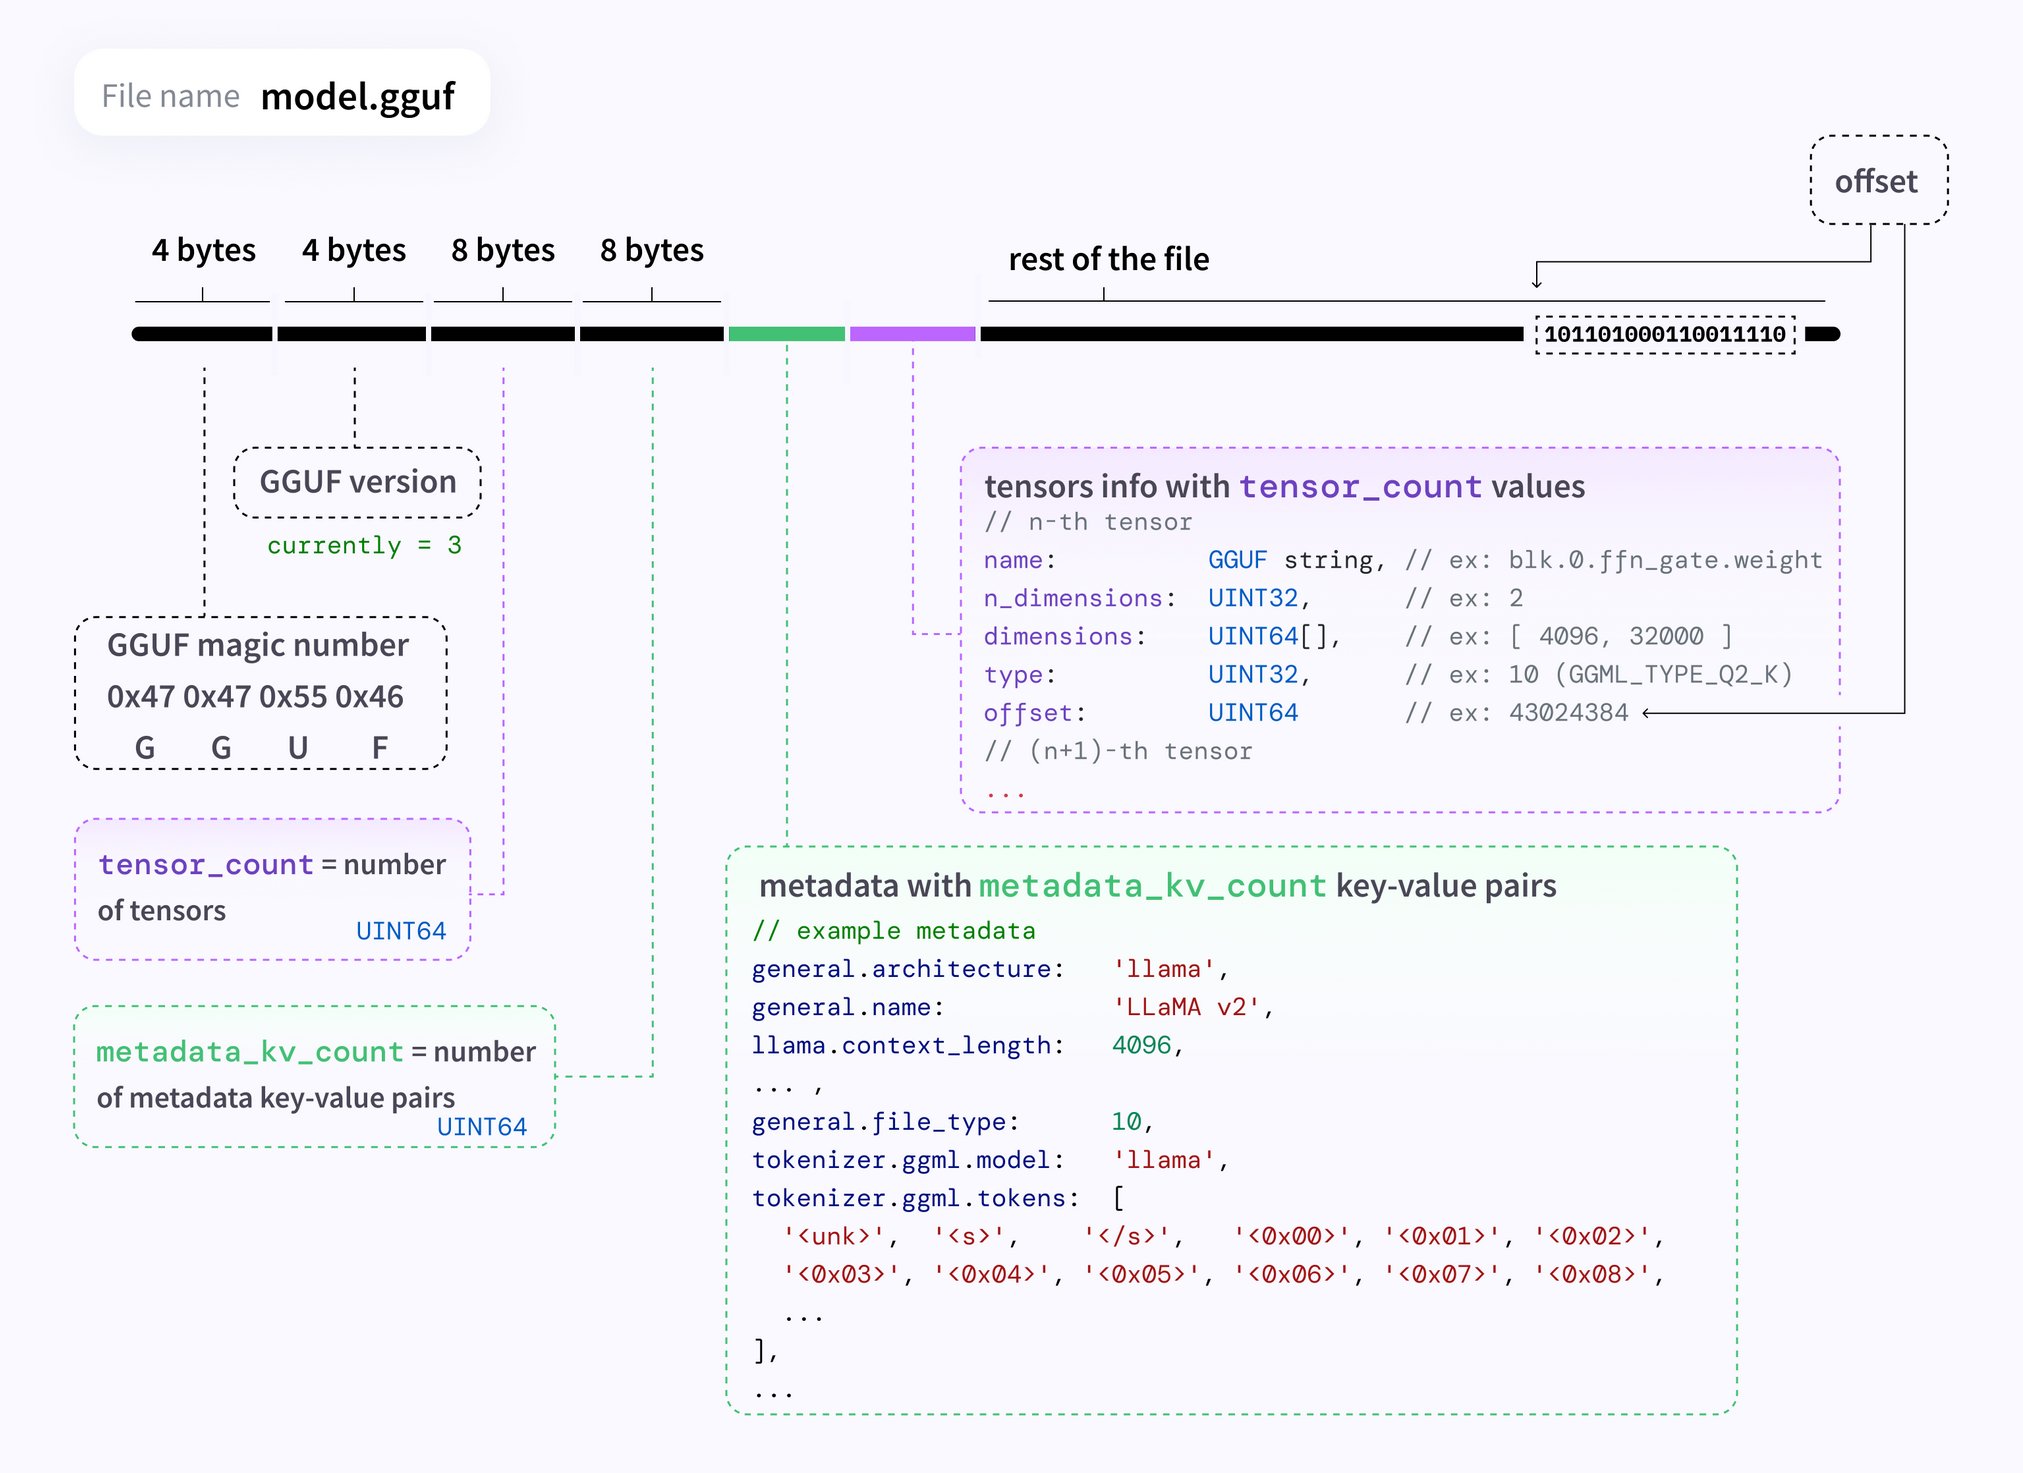
\includegraphics[width=\linewidth, height=0.45\textheight]{gguf}
			\captionof{figure}{GGUF Format Breakdown \cite{ggmlgithubdocs}}
			\label{fig:gguf}
		\end{minipage}
	\end{strip}
	
	\begin{strip}
		\begin{minipage}{\textwidth}\centering
			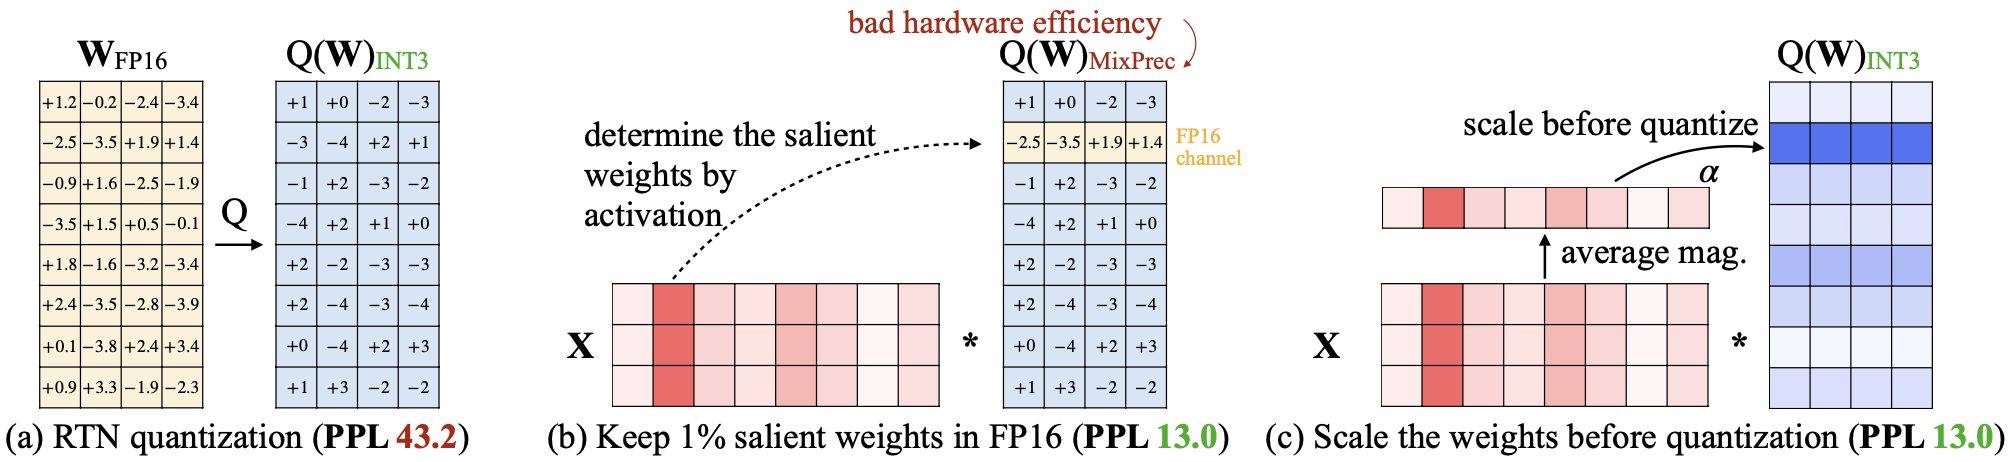
\includegraphics[width=\linewidth, height=0.2\textheight]{awq}
			\captionof{figure}{\gls{awq} method showing how scaling \textit{salient} weights before quantizations shows comparable results to mixed precision weights but without the hardware inefficiencies mix precision introduces \cite{lin2024awqactivationawareweightquantization}}
			\label{fig:awq}
		\end{minipage}
	\end{strip}
	
	The \texttt{llama.cpp} software developed by Georgi Gerganov and the open-source community is used to load the \gls{gguf} format. After it is loaded and processed based on the stored metadata, the underlying \gls{ggml} library can then begin inferencing the \gls{llm} \cite{ggufgithub}. The \gls{gguf} format offers various quantization options, originally the quantization method was to simply split each layer into blocks of 256 weights and each block is then converted into their 256 quantized values, this was demoted with a \textbf{Q}. Additionally, there are two quantization type, ``type-0" (\textbf{Q4\_0}, \textbf{Q5\_0}, etc) where weights $w$ are calculated from quants $q$ and block scale $d$ using $w = d * q$. While ``type-1" (\textbf{Q4\_1}, \textbf{Q5\_1}, etc) include an additional block minimum constant $m$ such that $w = d * q + m$ \cite{ggufgithubquantdoc, ggufgithubkquantpr}. 
	
	Later the community have developed the \textbf{K} Quants, which expand the quantization range to include 2-bit, 3-bit and 6-bit quantization and includes prioritization for certain weights over others (as denoted by suffixes like \textbf{Q3\_K\_S}, \textbf{Q3\_K\_M}, \textbf{Q3\_K\_L}) which leads to smaller models with less \gls{ppl} increase \cite{ggufgithubkquantpr}. The newest form of \gls{gguf} quants are the \textbf{I} Quants which added a new low bit quantization \cite{ggufgithubiquantpr} which is based on the QuIP\# paper \cite{tseng2024quipbetterllmquantization}, which suggests grouping even number of either positive or negative signed values into 8 quants, allowing sign information to be recorded using only 7 bits and if needed flipping the sign of the least important quants to maintain even count, while the magnitude of the 8 quant groups can be stored in a E8 lattice structure using 8 bits to record the grid point index \cite{ggufgithubiquantpr}. 
	
	\subsection{\gls{awq} \gls{ptq}}
	
	Similar to the \textbf{K} Quants of \gls{gguf}, the \gls{awq} method proposes a similar approach of selectively quantizing \gls{llm} weights depending on their importance by analysing the model activation patterns \cite{lin2024awqactivationawareweightquantization}. This method identifies \textit{salient} weights in the \gls{llm} that hold more importance to the \gls{llm} performance and withhold quantization for those weights, thereby avoiding significant performance degradation while reducing the model size. However, having  mixed precision weights is not hardware-efficient, it was found that scaling the weights before quantization mitigates this issue while still preserving the benefits (see figure \ref{fig:awq}).
	
	\subsection{\gls{vptq} \gls{ptq}}
	
	Similar to the \textbf{I} Quants of \gls{gguf}, the \gls{vptq} method is a low bit \gls{llm} quantization method that claims better accuracy for 1-2 bit \gls{llm} quantization compared to other conventional methods. It tries to achieve this by compressing vectors into indices by using lookup tables with additional refinement of weights using Channel-
	Independent Second-Order Optimization \cite{liu2024vptqextremelowbitvector}. It differs from the previously covered \gls{awq} method as instead of reducing precision of the weights, it builds an index that maps high-dimensional vectors to lower-dimensional vectors. According to the graph on figure \ref{fig:vptq}, it's performance is comparable to QuIP\# method which the \textbf{I} Quants of \gls{gguf} are based on.
	
	\begin{figure}[h]
		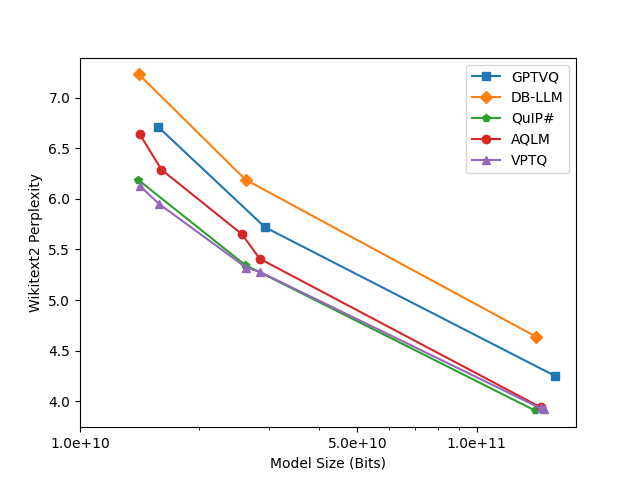
\includegraphics[width=1.1\linewidth]{vptq}
		\captionof{figure}{Graph showing \gls{ppl} of Wikitext2 dataset compared to model size using various \gls{ptq} methods \cite{vptqgithub}}
		\label{fig:vptq}
	\end{figure}
	
	\subsection{\gls{llm} Pruning}
	Model pruning is a way of compressing the size of a model by removing certain components from the model while avoiding severe damage to how the model functions. This is achieved by removing redundant or unimportant singular or groups of neurons \cite{huang2024largelanguagemodelpruning}. There are two type of pruning methods that can be performed on a model, structured pruning and unstructured pruning, the former involves simplifying the model by removing entire structural weights such as channels or layers while maintaining the network structures, while the latter focuses on removing redundant neurons or links \cite{huang2024largelanguagemodelpruning}. Between the two approaches, structured pruning has much better hardware compatibility compared to unstructured pruning which maybe require additional software or hardware treatment to complete the task \cite{huang2024largelanguagemodelpruning}.
	
	LLM-Pruner is a tool developed to perform structural pruning on an \gls{llm} using gradient-based optimization processes for structure selection \cite{ma2023llmprunerstructuralpruninglarge}. The LLM-Pruner uses an algorithm to detect dependencies within a model, this allows them to select optimal structured groups for pruning based on their importance estimation. Like with most pruning methods, a post pruning re-training is required, which can be called a ``recovery" phase, where it's trained on a small dataset in order to help maintain it's performance \cite{ma2023llmprunerstructuralpruninglarge}.
	
	Unlike LLM-Pruner, the Bonsai pruning method does not use a gradient-based structured pruning and is designed for more typical consumer grade hardware to execute \cite{dery2024everybodyprunenowstructured}. It instead generates sub-models and evaluates their performance to give a more holistic view, which claim to outperform \gls{sota} ``gradient-based structured pruning methods like LLM-Pruner" \cite[p.~2]{dery2024everybodyprunenowstructured} on 4/6 evaluation tests. Similar to LLM-Pruner, the Bonsai method performs post pruning operations to help recover some lost performance, but unlike LLM-Pruner, it uses distillation from the original model to the pruned model. However, in some cases this post pruning adaptation may not be necessary due to the robustness of the \gls{llm} as well as redundancy of its modules \cite{dery2024everybodyprunenowstructured}.
	
	\subsection{\gls{llm} Benchmarking}
	
	There are many benchmark dataset available that are designed to test for various capabilities of \glspl{llm}, and as mentioned in the research scope section, this research will focus on a subset of datasets from three categories of \textbf{General Knowledge and Language Understanding}, \textbf{Reasoning Capabilities}, \textbf{Truthfulness} and \textbf{Instruction Following}. Starting with \gls{mmlu} Pro dataset which is an iterative improvement over the original \gls{mmlu} dataset by removing trivial and noisy questions \cite{wang2024mmluprorobustchallengingmultitask}. It's a dataset with a diverse fields such as mathematics, computer science, physics, chemistry, biology, business and more to produce over 12,000 questions \cite{wang2024mmluprorobustchallengingmultitask}. The dataset is constructed as series of multiple choice questions with up to 10 possible response options, compared to only 4 in the original \gls{mmlu} dataset, which should reduce random guessing score \cite{mmluprohuggingface}.
	
	Next dataset to look at is HellaSwag, which similar to \gls{mmlu} part of the \textbf{General Knowledge and Language Understanding} category. This dataset evaluates an \glspl{llm} capability of answering questions in a contextually appropriate and common-sense manner, referred to as \textit{common-sense natural language inference} \cite{zellers2019hellaswagmachinereallyfinish}. Similar to \gls{mmlu} the dataset is structured as multiple choice questions.
	
	Moving onto the \textbf{Reasoning Capabilities} category, AGIEval dataset uses various human-centric exams to evaluate a models reasoning capabilities \cite{zhong2023agievalhumancentricbenchmarkevaluating}. The dataset is constructed with a particular focus on human-level cognitive tasks and real-world scenarios following a wide range of exam papers like mathematics exams, lawyer qualification tests, college admission tests and other qualification exams \cite[p.~5]{zhong2023agievalhumancentricbenchmarkevaluating}. The format of the dataset is comprised of multiple choice with an addition of some fill-in-the-blank questions that employ exact matching strategy during evaluation \cite[p.~6]{zhong2023agievalhumancentricbenchmarkevaluating}.
	
	For the \textbf{Truthfulness} category there exists a TruthfulQA dataset that evaluates a model for providing accurate and unbiased information. The benchmark consists of over 800 questions that covers 38 categories which include law, health, finance and politics \cite{lin2022truthfulqameasuringmodelsmimic}. This dataset was designed to help address the concerns of accidental and/or malicious \gls{llm} misuse. It relies heavily on true or false questions and uses Wikipedia to source the factual information. The questions in the dataset were designed to be adversarial such that ``questions test a weakness to imitative false-hoods: false statements with high likelihood on the training distribution" \cite[p.~4]{lin2022truthfulqameasuringmodelsmimic}
	
	Finally, for the \textbf{Instruction Following} there is the \gls{ifeval} dataset which was designed to evaluate how well a model follows a set of instructions in the prompt using verifiable instructions. A verifiable instruction is a specific, measurable and objective directive that, upon completion, can be checked and confirmed for adherence \cite{zhou2023instructionfollowingevaluationlargelanguage}. The \gls{ifeval} has identified 25 types of verifiable instructions and the dataset is comprised of 500 prompts based on those types. An example of such instruct prompt is ``write at least 25 sentence" which can be automatically and objectively verified \cite{zhou2023instructionfollowingevaluationlargelanguage}. This dataset is quite valuable as it stands to reason that a model that can follow instructions well will do better at answering multiple choice questions, which most of other previously mentioned datasets use, which require a certain level of structure in the response to be evaluated correctly.
	
	\subsection{Summary}
	This preliminary literature review section has explored some of the existing \gls{llm} \gls{ptq} methods such as \gls{gguf}, \gls{awq} and \gls{vptq}. All of the discussed methods operate based on similar principals of reducing the precision of the numeric values within the model weights. The \gls{gguf}, being a community driven open-source project has more options for quantization available to it in the form of \textbf{K} quants (which selectively quantize certain weights over others) and \textbf{I} quants (which is based on QuIP\# method involving clever sign grouping and E8 lattice structure storage). Following from this, the \gls{llm} pruning methods LLM-Pruner and Bonsai function by removing parts of the model which has little impact on it's quality. The differing feature between the two approaches lies with it's selection process for the structured groups (gradient-based versus sub-model evaluation). Finally, benchmarking review covered various datasets that evaluate specific model capabilities such as \textbf{General Knowledge and Language Understanding}, \textbf{Reasoning Capabilities}, \textbf{Truthfulness} and \textbf{Instruction Following}. 
	
	\section{Working Theory}
	Following from the preliminary literature review, this section will define \glspl{tp} based on the previously reviewed literature which will help guide this papers \glspl{rq}.
	
	\textbf{\gls{tp}1}: \textit{The effectiveness of \gls{ptq} techniques in reducing computational requirements is influenced by the \gls{llm} architecture, where certain architectures benefit more than others}.\\
	
	
	\textbf{\gls{tp}2}: \textit{The combination of \gls{ptq} and pruning can achieve significant reduction in hardware requirements compared to using only one approach over the other}.\\
	
	\textbf{\gls{tp}3}: \textit{The impacts of \gls{ptq} and pruning on \gls{llm} performance can vary across different types of tasks (e.g. Instruction Following, Reasoning, Knowledge) }.\\
	
	\textbf{\gls{tp}4}: \textit{An \glspl{llm} reasoning tasks will be more strongly impacted compared to knowledge retrieval tasks after applying a \gls{ptq} or pruning method}.\\
	
	
	\section{Research Design}
	\subsection{Introduction}
	\subsection{Design}
	
	\section{Conclusion}
	
	\bibliography{proposal}
	
	\printglossary[title={Glossary}]
	
	\appendix
	\section{Appendix A}
\end{document}
